\documentclass[]{article}

\usepackage{marginnote}
\usepackage{verbatim}
\usepackage[letterpaper,left=3cm,right=4cm]{geometry}

\usepackage{graphicx}

\usepackage{fancyhdr}
\pagestyle{fancy}

\usepackage[colorlinks=true]{hyperref}
\hypersetup{allcolors={blue}}
\hypersetup{pdftitle={Random Variable Functions}}
\hypersetup{pdfauthor={Paul Glezen}}
\hypersetup{pdfcreator={Latex}}
\hypersetup{pdfkeywords={ISAB, Workshop, Probability, Distributions}}

\setlength{\parindent}{0em}
\setlength{\parskip}{1em}

\title{Random Variable Functions}
\author{Los Angeles County\\ISAB}
\date{July 12, 2017}

\begin{document}
\maketitle

We've been discussing random variables, their CDF and PDF, and their
moment generating functions.  We've done a few exercises invovled with
calculating their means and variance.  The random variables we've discussed
so far directly modeled certain phenomena, such as a coin flip, the number
of heads in multiple coin flips, and selecting a number randomly from a set
of numbers.  This is all very nice; but it's time to step up our game and
consider random variables that arise as a function of other random variables.

Let's remind ourselves of what a random variable is.
A random variable maps from an abstract event space to points on
the real number line.  Often the event space won't be so abstract
and the mapping will be quite natural; so natural that we often just
write $X$ rather than
$X(\omega) \in \mathcal{R}$ for $\omega \in \Omega$.

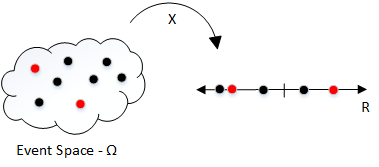
\includegraphics[width=\linewidth]{rv1.png}

By mapping from ``event spaces'' to the concrete real number line,
random variables allow us to directly employ analytic techniques
that have long existed for the real number line.  Our
cumulative distribution functions and probability density functions
are defined on the real number line by virtue of the random variable
mapping events to the real number line.

A function of a random variable simply maps the points from one
real number line to another real number line.  In this way, a function
of a random variable creates a new random variable on the same event
space, i.e. a new way to map events to real numbers.

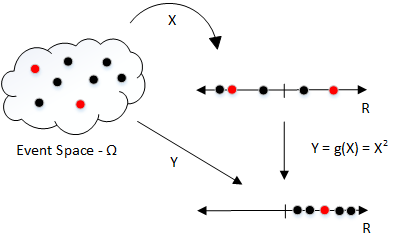
\includegraphics[width=\linewidth]{rv2.png}

In the figure above, $g(x) = x^2$ is such a function.  If we define
$Y$ as the result of mapping
$\Omega \rightarrow \mathcal{R} \rightarrow \mathcal{R}$, then
$Y$ is also a random variable.

Assuming that such a mapping is useful (and we'll find out later that
this $g(X) = X^2$ is), we'll want to know the CDF and PDF of the new
random variable.  Unfortunately, it's not as simply as plugging
$x^2$ everywhere you see an $x$.

Using the figure above as an example, let's determine $F_Y(y)$ from
basic principles.  The basic principle is

$$
F_Y(y) = P[Y \le y]
$$

From this principle we plug in the function to derive the expression.
Since $Y = g(X) = X^2$, we restrict our attention to $y > 0$ since
$F_Y(y) = 0$ for $y \le 0$.

\begin{eqnarray*}
F_Y(y) &= &P[Y \le y] \\
  &= &P[X^2 \le y] \\
  &= &P\left[-\sqrt{y} \le X \le \sqrt{y}\right] \\
  &= &P\left[X \le \sqrt{y}\right] - P\left[X \le -\sqrt{y}\right]
\end{eqnarray*}

This gives us the CDF for Y.  It's close to simply substituting
$\sqrt{y}$ for $x$ into the expression for $F_X$.  Now that we have
the CDF, we can derive the PDF.

\begin{eqnarray*}
f_Y(y) &= &\frac{d}{dy}F_Y(y) \\
   &= &\frac{d}{dy}\left[ F_x(\sqrt{y}) - F_X(-\sqrt{y}) \right] \\
   &= &\left. \frac{dF_X}{dx} \right\vert_{x=\sqrt{y}} \frac{d(\sqrt{y})}{dy} - 
   \left. \frac{dF_X}{dx} \right \vert_{x=-\sqrt{y}} \frac{d(-\sqrt{y})}{dy} \\
   &= &\frac{1}{2\sqrt{y}} \left[ f_x(\sqrt{y}) + f_x(-\sqrt{y}) \right]
\end{eqnarray*}

where

$$
\frac{dx}{dy} = \frac{d y^{\frac{1}{2}}}{dy} = \frac{1}{2}y^{-\frac{1}{2}}
$$

The expression for $f_Y$ in terms of $f_X$ in this specific case of
$Y = X^2$ demonstrates two important complications.

1. If $g$ is not 1-to-1, then we must account for all the points
   in $g^{-1}(y)$.  In the case of a quadratic, there are usually
   two.

2. The $f_Y$ expression introduced an additional multiplicative
   factor, known in calculus circles as \emph{the Jacobian}.  The
   Jacobian incorporates the stretch factor introduced by the
   transformation.

It's reasonable to ask why the CDF didn't need a stretch factor.
It's because we don't integrate the CDF.  We just evaluate it at
various points.
\textbf{The value of the CDF at any point represents a probability.}

This is not the case with a continuous density function.  The
value of $f_X$ at point does not really mean anything
\textbf{by itself.
It certainly does not represent a probability.}  We only get
probabilities from $f_X$ by integrating it over some interval
or combination of intervals.  In other words, it's only the
area under $f_X$ that has a probability interpretation.  You
can't say anything about an area with just the height.  You
need to also specify the width.  So in the case of our transformation
$g$, it's not enough to determine the height of $f_Y$ at a certain
point through corresponding values of $f_X$.  We need to know how
$g$ is stretching the differential widths to get the full picture
of how areas under $f_X$ transform to \emph{areas} under $f_Y$.  The
Jacobian factor provides this ``width stretching'' information.

We're still messing around in the realm of probability.  In the next
workshop, we'll consider some special functions of a random
variable (like the average of a sample) and cross into the
realm of \emph{statistics} proper.


\end{document}  